\section{More Event-B Features}\label{features}
Event-B is based on the Rodin, open-source, project. There are two distinct sets of plug-ins: firstly there are a set of core plug-ins, which is mostly maintained, and coordinated, by a commercial organization; and there are a number of open-source plug-ins, some maintained by the commercial organization, others by academic institutions, or jointly. Section.~\ref{intro} gave details of Event-B features provided by the core plug-ins. In this section we describe some important plug-in from the second category, namely Composition, Decomposition and the Theory plug-ins features. 
\subsection{Decomposition and Composition}

Decomposition and composition are two related approaches, that we use to partition a system, to allow us to work on smaller, manageable sub-models. Figure~\ref{fig:decomp2} illustrates the shared-event decomposition approach~\cite{decomp2010c} which we make use of in our code generation approach. An alternative shared-variable approach is described in~\cite{AbrialH07}. \emph{v1} and \emph{v2} are disjoint sets of variables, and \emph{p} and \emph{q} are disjoint sets of parameters. \emph{g} and \emph{a} are guards and actions that range over the  variables and parameters. In the shared-event decomposition approach the system is partitioned so that each variable is allocated to a single machine. In Fig.~\ref{fig:decomp2}, the variables of machine $m$ are partitioned into the sets $v1$ and $v2$ and decomposed into $m_a$ and $m_b$ respectively. The decomposed events have guards and actions which involve their respective variable partitions. The composed machine construct contains references to the decomposed machines. It keeps track of the refinement relationship between the abstract machine and the decomposed machines. In the decomposition, it is the synchronization of events, in different decomposed machines, that refines a single abstract event. 

The main purpose of using this form of event decomposition is that it reduces the size of the models, therefore making modelling and proof easier. The decomposed machines can be refined without restriction. For code generation, the synchronization of events provides a suitable basis for modelling procedures and procedure calls.
 %
\begin{figure}
\centering
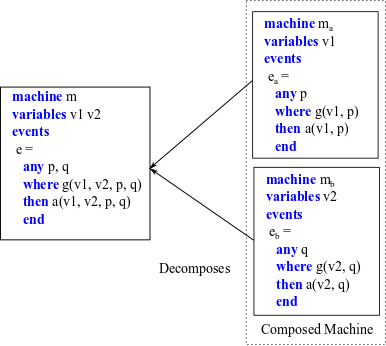
\includegraphics[width=0.5\textwidth]{graphics/Decomp2.png}
\caption{Decomposition}
\label{fig:decomp2}
\end{figure}
%
\subsection{Theories}
The theory plug-in provides a mechanism for extending the Event-B proof capabilities, and addition of new mathematical types~\cite{issam2013}. Proof obligations will be generated to verify the soundness of the augmented prover. We can make use of the following sections in the theory plug-in.

\begin{enumerate}
\item Type Parameters: A theory can define type parameters to be used as polymorphic types.
\item Datatypes: Used to define simple data types, which can be added using a type constructor and element constuctors.
\item Operators: The operators section can be used to define polymorphic operators, such as the sequence described as an ordered list~\cite{issam2013}. 
\item Axiomatic Definitions: These are defined to produce types, when no suitable type constructors or datatypes can be used as a basis for construction.
\item Theorems: Polymorphic theorems can be used to assist with the proof of newly introduced definitions. 
\item Rewrite rules: Rewrite rules define how to rewrite formulas to equivalent forms. When a rewrite rule is defined, the author specifies whether the rule should be applied automatically, or during an interactive proof session.
\item Inference rules: Rules are matched against sequent goals. If a match is found, a backward proof step is performed. The rule may also match a hypotheses of a sequent, where a forward proof step is performed.
\end{enumerate}


\subsection{Background for Code-Generation}
In the section so far we have looked at a number of other features of Event-B that will be used in the code generation approach. Decomposition provides the basic structuring of a development, that makes an Event-B development amenable to our code generation approach. We also make use of the theory plug-in by extending it to allow definition of translations from the Event-B mathematical language, to programming language mathematical expressions and conditions. We can also introduce more concrete data types, such as arrays, and provide translation details for these. 

\subsection{Targets for Code-Generation}\label{targets}
In this subsection, we provide details of the target languages that we wish to generate code for. Ada provided the original basis for the code-generation approach described in~\cite{Edmunds2012a} because its programming constructs are well defined and map well to Event-B. Ada tasks are processing units, known to the run-time system. Protected objects provide an encapsulation mechanism, that prevents interference in situations where data must be shared between concurrently executing tasks. In Java the processing unit is provided by Thread class, and encapsulation is provided by synchronized methods and blocks. In C, there is some choice about the method of thread implementation, such as OpenMP~\cite{openmp} threads, or POSIX threads\cite{pthreads}. In its most basic form, the encapsulation mechanism for protected regions must be coded explicitly. Our final code-generation target arises from our work on co-simulation of Cyber-Phsyical systems in the Advance project~\cite{advance}. In this approach we generate a specialized form of C code, conforming to the FMI standard for model co-simulation~\cite{FMISTD}. This can be used to simulate the software running on an embedded controller, in a simulation of its environment.   
%
\begin{figure}
\centering
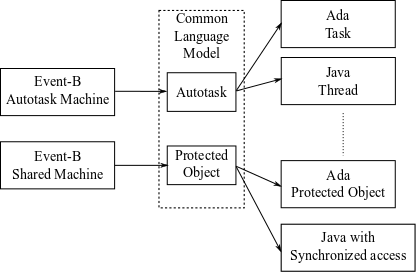
\includegraphics[width=0.6\textwidth]{graphics/B_IL1_others.png}
\caption{The Common-Language Model}
\label{fig:B_IL1_others}
\end{figure}
%
In order to provide some commonality in the code generation process we formulated a two-stage code-generation process, as shown in Fig.~\ref{fig:B_IL1_others}, which is a modified from Fig.~\ref{fig:B_Ada}; where the first step is a translation to a common-language model, which is an abstraction of the required implementation. The second stage is a back-end processor, translating to the various target implementation languages. The semantics of the common-language model are formulated using Event-B, and provides a formal basis for the translation. We will discuss the semantics of Tasking Event-B in Sect.~\ref{TEB}.
